\documentclass[12pt, a4paper]{article}

% Structural
\usepackage[margin=1in]{geometry}
\usepackage[english]{babel}
\usepackage[utf8]{inputenc}
\pagenumbering{arabic}

% Packages
\usepackage{amsmath}
\usepackage{amssymb}
\usepackage{graphicx}
\usepackage{wrapfig}
\usepackage{titlesec}

% Title
\title{Analysis of 2 Different classifiers of CIFAR-10 Dataset}
\date{December 7, 2019}
\author{Beomjun Bae, Alexis Romero, and Octavi Obiols Sales\\
CS271 - Machine Learning\\
Final Project Report}

\begin{document}
	\maketitle
	\section{About CIFAR10 Dataset}
		CIFAR-10 dataset is a commonly used benchmark dataset in the image categorization community, and its popularity can be attributed to 3 of its properties: ease of use, availability, and level of variability. CIFAR10 dataset is easy to use, because it is already labeled into 10 different categories. Here is a visualization of the images organized by categories by row:\\
		\centerline{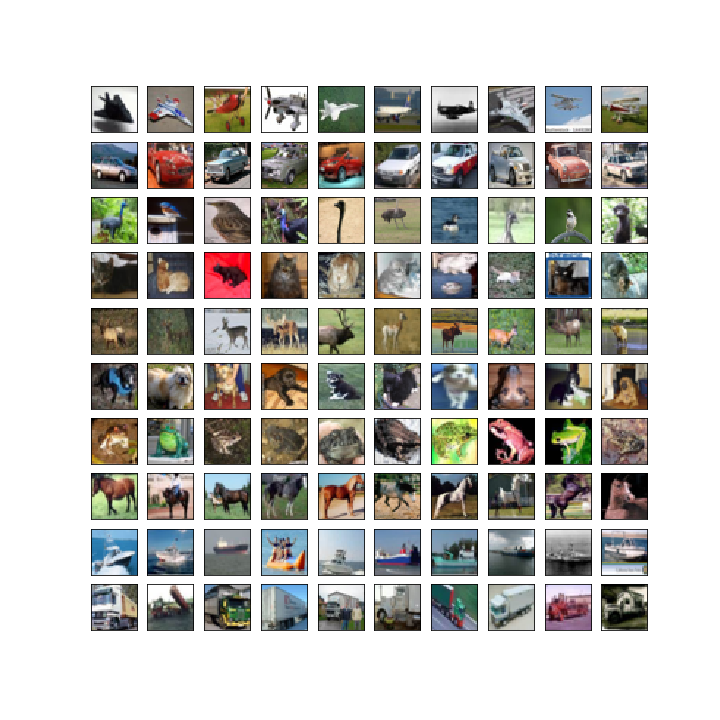
\includegraphics[width=4in]{../figures/cifar10_organized.png}}
		Note that the first row only contains airplanes, the second, cars, and so on. There are a lot of images available for the researchers to use, but not many have a them labeled into 10 distinct categories. Because of the fact that the images are labeled, it leads well into making analysis using supervised machine learning models.\\
		Its availability is crucial as well. The data set has 6000 images per category which adds up to 60,000 total images. On top of the sheer abundance of the image set, the image comes already reshaped into 60,000 by 32 by 32 by 3 format. 32 by 32 because of the image size, and 3 because of each RGB channels of the image. Lastly, it is easy to find and use the dataset, because the author of the dataset Alex Krizhevsky made it publicly available.\\
		Lastly, CIFAR-10's level of variability is important as well. In comparison to other dataset, CIFAR-10 allows for a higher level of challenge. The standard before CIFAR-10 was MNIST handwritten digit database, and the reason it went out of style was because it was too easy to categorize. Machine learning models were achieving upwards of 90\% accuracy, and there simply wasn't enough room for improvement for next generation of machine learning models. However, CIFAR-10 has objects along with its background. This forces the models to be more intelligent which leaves enough room for improvement.
	\section{Project Goal}
		In our project, we attempt to compare and analyze the difference between two categorical models, Support Vector Machines and Multi-Layered Neural Network. The reason why we began looking into these two models is because of the type of the dataset that CIFAR-10 provides.\\
		As we mentioned above, CIFAR-10 dataset is an image dataset with 60000x32x32x3 format. But if we were to flatten the dataset, we get 60000x3027. Using this 2 dimensional form, we can pretend that the image data is just a simple vector for every label ranging from $[0,9]$. Now, we know that Support Vector Machines have the property of finding the best decision boundary given the feature vectors. Since we can represent the image information in a vector, we decided to create a classification with SVM.\\
		Secondly, since this is an image data, we decided to use a Convolutional Neural Network. This method is very appropriate for image classification, because convolution allows for identifying lower level features from the images. Furthermore, if we layer different convolutional networks, we can proceed to get a higher level features as well.\\
		Our goal is to see if the simple Support Vector Machine has the enough freedom with the hyperplane to appropriately classify the image dataset.
	\section{Support Vector Machine}
		Support vector machines finds the best decision boundary with the biggest margin between the two datasets. However, there are multiple different design decisions that we must make even within the frame work of SVM algorithm, and here are the 2 decision we want to highlight:
		\subsection{Modeling Decisions}
			\subsubsection{Linear over Complex Kernel Function}
				\begin{wrapfigure}{r}{0.5\linewidth}
					\centering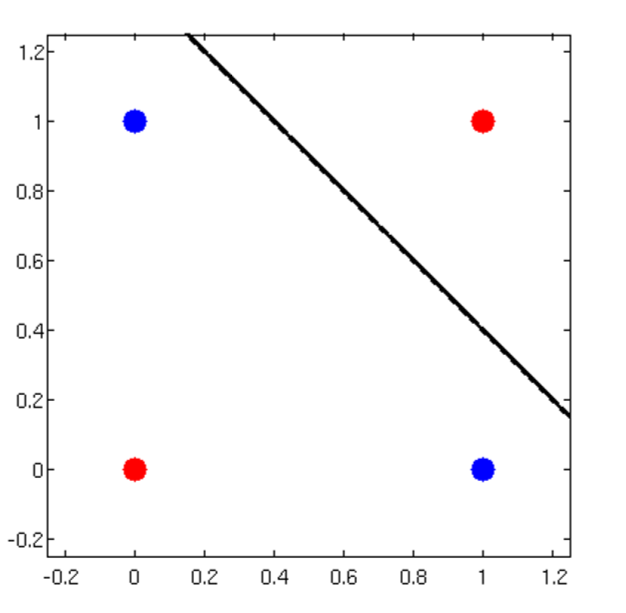
\includegraphics[width=0.5\linewidth]{../figures/xor.png}
				\end{wrapfigure}
				The single most important aspect of Support Vector Machine's success might be the kernel function. This is because it provides the freedom SVM needs to classify the data points affectively. Look at the classic case of XOR diagrammed here. We can clearly see that linear classifier simply does not have the freedom it needs to classify the dataset perfectly. However, if we were to use more flexible kernels like radial basis function or a polynomial kernel, we would be able to classify without error.\\\\
				However, accuracy is not the only concern in our case. We realize that when we use a non-linear kernels, we need to trade off the training time for the accuracy. Because the kernel matrix needs to be calculated for every pair of data point, we realize that the costs is $O(n^2)$ at the least and $O(n^3)$ at the worst. With the CIFAR-10 dataset containing 60,000 data points, we simply could not afford to use a complex kernel function given the timeline of our project report. Instead, by using a linear kernel, we calculate the dot product of the dataset on the fly, which makes the algorithm much more efficient.
			\subsubsection{Multi-class decision making Strategy}
				CIFAR-10 dataset has multiple classes that label the images. Therefore, the standard support vector classification methods have a hard time, because it is built on the assumption that the data point that lie above the decision boundary is positive and below is negative. Thus, in order to convert this into a multi-class classifier, we need to train multiple classifiers that can identify each class.\\\\
				There are two main strategies: One versus One or One verses Rest. One versus One strategy requires that we filter the total samples into two chosen classes, and classify accordingly. As you can see we will have ${10\choose 2}=45$ different ways of choosing a pair. This means that we will have to train the SVC 45 different times. We decided that this strategy is unrealistic given our timeline of the project, so we pursued the second strategy.\\\\
				The One verses Rest strategy only requires us to train 10 different classifiers, because we train considering non-chosen classes as negative classes. The only drawback of this strategy is that it will cause an imbalance of data points, which may affect the accuracy of the model.
		\subsection{Data Manipulation Decisions}
			Our flattened data set is in the dimension 60,000 by 3072. Given this large dataset, we decided to shrink the size of the matrix by performing PCA, and ultimately reduce the number of features given an image. The results below will show you how the number of features affects thte results of the SVC.
		\subsection{Validation Results}
			First, results from Support Vector Classifier with pretty small number of features, $m=500$, we get the following result:
			\centering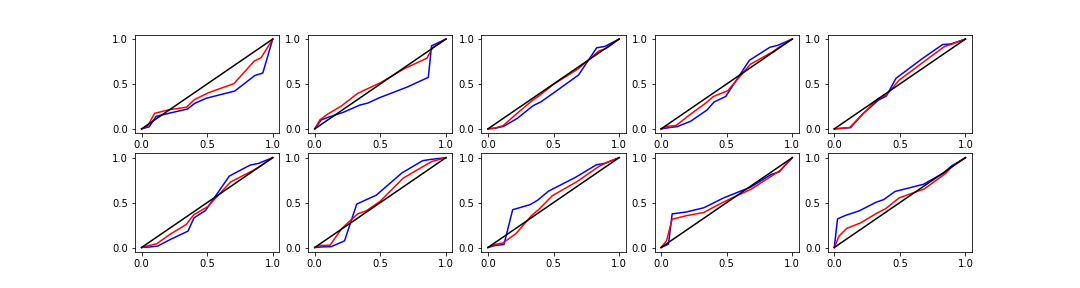
\includegraphics[width=7in]{../figures/roc_curve_pca500.png}\\
			Above is a plot of the ROC curve of each class ranging from $[0,9]$. The blue line represents the result on the training data, and the red line represents the one on the test data. Notices that for the most part, the model performs not much better than the 50\% guessing line. We suspected that this must be because it does not have enough features. Therefore, we increase the number of features to $m=1500$:
			\centering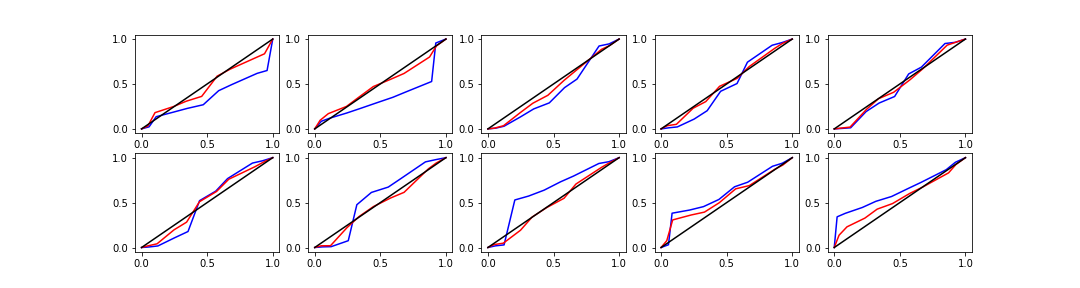
\includegraphics[width=7in]{../figures/roc_curve_pca1500.png}\\			
			Notice that the results still have yet to improve much. Here, we conclude that the number of features is not the determining factor. Also, we conclude that linear support vector classifiers have hard time classifying the images.
	\section{Multi-Layered Neural Network}
	\section{Conclusion}
\end{document}